
```{tikz }
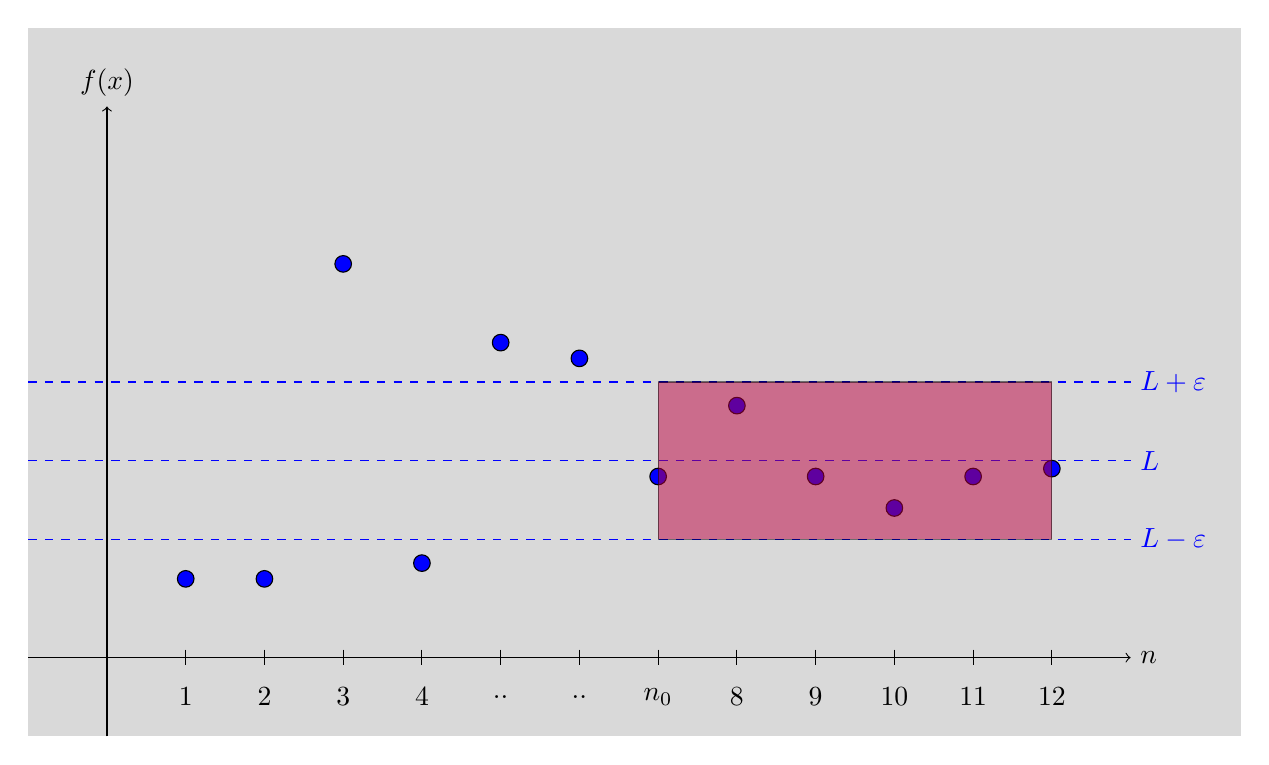
\begin{tikzpicture}
\fill[gray!30] (-1,-1) rectangle (14.4,8);
\draw[->] (-1,0) -- (13,0) node[right] {$n$};
\draw[->] (0,-1) -- (0,7) node[above] {$f(x)$};
\draw[dashed,blue] (-1,3.5) -- (13,3.5) node[right] {$L+\varepsilon$};
\draw[dashed,blue] (-1,2.5) -- (13,2.5) node[right] {$L$};
\draw[dashed,blue] (-1,1.5) -- (13,1.5) node[right] {$L-\varepsilon$};
\foreach \point in {(1,1), (2,1), (3,5), (4,1.2), (5,4), (6,3.8), (7,2.3), (8,3.2), (9,2.3), (10,1.9), (11,2.3), (12,2.4)} {
    \draw[fill=blue] \point circle (3pt);  
}
\draw[fill=purple,opacity=0.5] (7,1.5) rectangle (12,3.5);

\foreach \x/\n in {1/1, 2/2, 3/3, 4/4, 5/.. , 6/.., 7/n_0, 8/8 , 9/9 , 10/10, 11/11 , 12/12} {
    \node at (\x,-0.5) {$\n$};
    \draw (\x,0.1) -- (\x,-0.1);
}
\end{tikzpicture}
```



